\section{Section Title}
\subsection{Problem}
Traditional \cite{hasanIntrinsicCompressibilityEffects2025,modestiReynoldsMachNumber2016} and \cite{morkovin1962effects,popeTurbulentFlows2000,trettelMeanVelocityScaling2016} studies of turbulence on incompressible flows led to important scaling relationships that define the flow in different regions. These regions are displayed in \Cref{fig:wall-regions}. In particular are the viscous sublayer and log-law region, which have empirical relations known as the law of the wall and log law. From these known relations, researchers can check that they are capturing the relevant turbulence scales in their experiments or simulations. It is also used to back out shear stresses and approximate friction and heat transfer coefficients as well as develop turbulence models. In computational fluid dynamics (CFD) simulations, these relations are used to develop wall functions that can be evaluated in the wall region, instead of fully resolving the wall region with spatial discretization.

\begin{figure}[h]
  \centering
  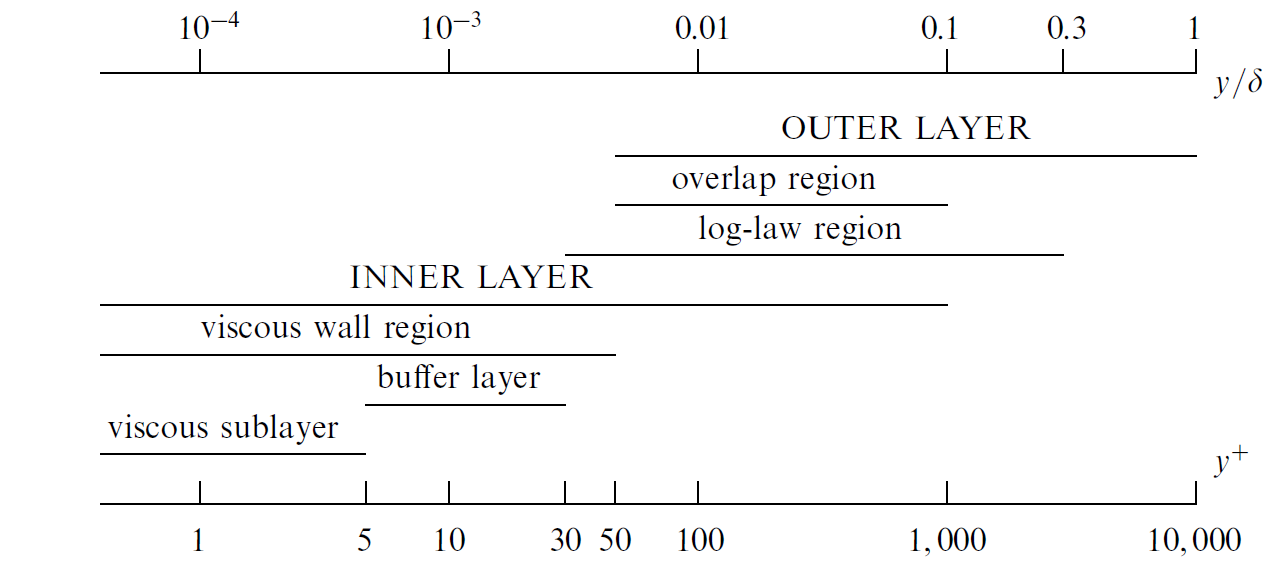
\includegraphics[width=.75\textwidth]{images/wall-regions.png}
  \caption{Depiction of wall regions at different $y^+$ from Pope \cite{popeTurbulentFlows2000}}
  \label{fig:wall-regions}
\end{figure}

There are many excellent tools and methodologies for incompressible turbulent flows that utilize the law of the wall and log law concepts. Ideally, we would want to reuse what has been developed for incompressible turbulence and apply it to compressible turbulence. To do this, an equivalent law of the wall and log law must be derived for compressible turbulence. This is done through a transformation of variables. The historical Van Driest transformation \cite{vandriestTurbulentBoundaryLayer1951} is one such transformation that aimed to achieve this and is still used by researchers to this day. While the Van Driest transformation performs excellently for adiabatic walls, it performs poorly for isothermal walls. The transformation should collapse the compressible velocity profiles onto the incompressible ones. \Cref{fig:vd} demonstrates this concept and how the Van Driest transformation performs for isothermal walls.

\begin{figure}[h]
  \centering
  \vspace{5pt}
  \begin{overpic}[width=.40\textwidth]{images/vdleg1.png}
    \put(35,-5){(a) Adiabatic}
  \end{overpic}
  \quad
  \begin{overpic}[width=.40\textwidth]{images/vdleg2.png}
    \put(35,-5){(b) Isothermal}
  \end{overpic}
  \setlength{\abovecaptionskip}{20pt}
  \caption{\label{fig:vd} Comparison of compressible (colored lines and symbols) to incompressible (solid black) turbulence using Van Driest transformation taken from Trettel \& Larsson \cite{trettelMeanVelocityScaling2016}}
\end{figure}

\subsection{Transformations}
The effects of compressibility on turbulence are typically split into indirect and genuine compressible effects. Indirect effects are due to mean density and temperature variations while genuine effects are caused by dilatational velocity fluctuations and thermodynamic fluctuations. Morkovin \cite{morkovin1962effects} hypothesized that if indirect compressibility effects are properly accounted for, the compressible turbulence distributions should collapse back to their incompressible forms. This hypothesis has been well validated by many experiments and simulations \cite{modestiReynoldsMachNumber2016}. Genuine compressibility effects start to matter at hypersonic (M~$\gtrsim$~5) conditions.

A key feature of compressible flows is that density is no longer constant, that is, $\rho$ and variables that depend on it in the original $y^+$ equation are no longer constant throughout the flow. The famous Van Driest transformation \cite{vandriestTurbulentBoundaryLayer1951} adjusts the velocity gradient, $\frac{du}{dy}$, to match log layer scaling. The transformed velocity then yields a transformed $u^+$. Van Driest chose to evaluate $\rho$ dependent terms at the wall; this yields a transformed $y^+$. The Van Driest transformed wall distance and nondimensional velocity are shown in \Cref{eqn:vd1} and \Cref{eqn:vd2}, where the $u^+$ in \Cref{eqn:vd1} is the untransformed $u^+$ with $u_\tau$ evaluated at the wall.

\begin{align} %van-driest
  U^+_{VD} & = \int^{u^+}_0 \sqrt{\frac{\langle\rho\rangle}{\langle\rho_w\rangle}}du^+ \label{eqn:vd1} \\[0.5ex]
  Y^+_{VD} & = \frac{(u_\tau)_w y}{\nu_w} \label{eqn:vd2}
\end{align}

Trettel \& Larsson formulated an improved compressibility transformation \cite{trettelMeanVelocityScaling2016} by assuming Morkovin's scaling applies everywhere in the flow. Prior researchers made similar transformations based on Morkovin's scaling, but other assumptions were also used, such as the Reynolds stress being zero in the viscous sublayer. Trettel \& Larsson don't use any other assumptions in their transformation derivation. The resulting transformation of $u^+$ and $y^+$ from their stress balance and scaling arguments are displayed in \Cref{eqn:tl1} and \Cref{eqn:tl2}. Compare to \Cref{eqn:vd1} and \Cref{eqn:vd2} and notice that local evaluations of density are used, and a more complicated $u^+$ equation is derived. We will see how much more powerful this transformation is.

\begin{align} %TL
  U^+_{TL} & = \int^{u^+}_0 \sqrt{\frac{\langle\rho\rangle}{\langle\rho_w\rangle}} \left[1 + .5\frac{1}{\langle \rho \rangle} \frac{d \langle \rho \rangle}{dy} y-\frac{1}{\langle \mu \rangle}\frac{d \langle \mu \rangle}{dy}y \right]du^+ \label{eqn:tl1} \\[0.5ex]
  Y^+      & = \frac{u_\tau(y) y}{\nu(y)} \label{eqn:tl2}
\end{align}